\documentclass{report}
\usepackage[utf8]{inputenc}
\usepackage[T1]{fontenc} 
\usepackage[francais]{babel}
\usepackage{colortbl}
\usepackage{amssymb}
\usepackage{pgf, tikz}
\usepackage{xcolor}
\usepackage{array}
    \title{\textit{Rapport} \\ La compression}
    \author{Lucas \textsc{Labadens} \and Isabelle \textsc{Marino} }
    \date{Le \today}
\begin{document}
\maketitle
 

\section*{Introduction}
La compression de données ou codage de source est un processus informatique permettant de transformer un document sous forme binaire en un autre document du même contenant une suite de bit plus courte que le précédent mais pouvant restituer les mêmes informations en utilisant un algorithme de décompression propre à algorithme de compression qui fut utilisé. En d'autres termes, la compression raccourcit la taille des données. La décompression est l'opération inverse de la compression.

Il y a notamment 2 grands types de compression:
\begin{itemize}
\item la compression sans perte de données
\item la compression avec perte de données
\end{itemize}

Un algorithme de compression sans perte restitue après compression et décompression un document strictement identique à l'original. Les algorithmes de compression sans perte sont utiles pour les documents, les archives, les fichiers exécutables ou les fichiers textes.
Pour la compression de données sans perte, on distingue principalement deux types de codage : le codage entropique et le codage algorithmique.

Avec un algorithme de compression avec perte, la suite de bits obtenue après les  compression et décompression est différente de l'originale, mais l'information restituée est très proche. Les algorithmes de compression avec perte sont utiles pour les images, le son et la vidéo.

Les formats de données tels que ZIP, RAR, GZIP, MP3 et JPEG utilisent des algorithmes de compression de données.
La compression est un procédé très utilisé dans la vie courante pour, par exemple, envoyer certains documents par e-mails ou pour le skockage de documents sur disque dur ou cloud center.
  
Le but de notre projet est de compresser des fichiers sans perte de données. 
Nous allons donc vous présenter différents algorithmes de compression sans perte de données que nous avons coder puis tester.

Dans un premier temps nous vous présenterons, entre autre, le codage de Huffman statique et celui de Lempel-Ziv. 
Pour cela nous avons choisit d'utiliser le langage Java pour nous permettre d'avoir des classes structurées et codées les différents algorithmes tout en gardant une structure et des fonctions communes.
 \part*{Algorithme de compression}
\chapter*{Huffman statique}
\section*{Définition et Exemple }
\subsubsection*{Défnition}
L'algorithme d'huffman statique est un algorithme de compression qui repose sur la redondance des caractères.En effet dans un fichier certain caractère sont plus présent que d'autre par exemple dans un fichier texte en français on retrouve souvent beaucoup de 'e' et 'a' mais très peu de 'w'.Un caractère étant codé sur octet l'algorithme d'huffman code un caractère non plus sur un octet mais sur un nombre de bit,plus le caractère est récurent plus le nombre de bit utilisé pour l'encoder sera faible.Cette algorithme neccéssité deux lecutres du fichier pour compresser,une pour compter les caracères l'autre pour écrire la compression,mais il permet à la décompression d'avoir déjà accès au codage propre a chaque lettre.Pour cela on utilise un arbre binaire.On compte le nombre de fois qu'apparait un caractère dans un fichier et ce nombre sont poids.Une fois l'ensemble des caractères du fichier comptez.L'ensemble des caractères muni de leur poids constitueront les feuilles de l'arbre de compression.On relie ensuite les deux feuilles les plus faibles avec un node intermédiaire qui aura pour poids la somme des poids de ces deux feuille, puis l'on répète l'opération avec les feuilles restante en reliant toujours les deux poids les plus faibles.Puis l'on relie les nodes racines entre elle toujours en reliant d'abord les plus faibles jusqu'a ne plus avoir qu'un seul et unique arbre. Ainsi chaque feuille ayant un chemin unique celui servira de code pour le caractère.En partant de la racine si l'on va au fils gauche on ajoute le bit 0 et si l'on va vers le fils droit on ajoute le bit 1. Ainsi les caractère les plus redondants se trouvant en haut de l'arbre ,ils seront codé sur très peu de bit.
\subsection*{Compression}
Pour cela on utilise un arbre binaire.On compte le nombre de fois qu'apparait un caractère dans un fichier et ce nombre sont poids.Une fois l'ensemble des caractères du fichier comptez.L'ensemble des caractères muni de leur poids constitueront les feuilles de l'arbre de compression.On relie ensuite les deux feuilles les plus faibles avec un node intermédiaire qui aura pour poids la somme des poids de ces deux feuille, puis l'on répète l'opération avec les feuilles restante en reliant toujours les deux poids les plus faibles.Puis l'on crée un nouvel arbre en fusionnant les deux arbres ayant les racines de poids plus faible et à ce nouvel arbre on le fusionne avec l'arbre qui possède la racine de poids la plus faible et réitère l'opération jusqu'a qu'il ne reste aucun autre arbre.L'arbre obtenue suite à cela constituera notre arbre de compression. Ainsi chaque feuille ayant un chemin unique celui servira de code pour le caractère.En partant de la racine si l'on va au fils gauche on ajoute le bit 0 et si l'on va vers le fils droit on ajoute le bit 1. Ainsi les caractère les plus redondants se trouvant en haut de l'arbre ,ils seront codé sur très peu de bit.On écrit ensuite l'arbre de compression au début du fichier de compression.Puis on relis le fichier à comprimer en réécrivant chaque caractère avec leur nouveaux code dans le fichier de comprimé.
\subsection*{Decompression}
Pour décompresser un fichier comprimer avec l'algorithme d'Huffman statique,il suffit de récupérer l'arbre écrit en début de fichier puis de lire le fichier bit à bit.Si le bit lu est un 0 on se déplace à gauche dans l'arbre et à droite si c'est 1.Lorsqu'on arrive sur une feuille on écrit le caractère correspondant à cette feuille puis l'on retourne à la racine et on recommence l'opération jusqu'à avoir lu entièrement le fichier comprimer.Le chemin menant à une feuille étant unique on retrouve exactement le même fichier qu'au départ.
\subsection*{Exemple}
Prenons un fichier où il est écrit "fanfaronner".Les carctères présent sont 'f','a','r','o',et 'e'.Pour l'instant chaque caractère est codé sur un octet donc le mot pèse 11 octet soit 88 bit.
On crée ensuite une feuille pour chaque caractère que l'on trie par ordre croissant de répétition :
\begin{center}
(o,1) (e,1) (f,2) (a,2) (r,2) (n,3)
\end{center}
On relie ensuite les plus faibles entre eux :
\begin{center}
\begin{tikzpicture}
\node (0) at (0,0) {2};
\node (1) at (-1,-1) {(o,1)};
\node (2) at (1,-1) {(e,1)};
\node (3) at (4,0) {4};
\node (4) at (3,-1) {(f,2)};
\node (5) at (5,-1) {(a,2)};
\node(6) at (8,0) {5};
\node(7) at (7,-1) {(r,2)};
\node(8) at(9,-1) {(n,3)};
\draw [-,>=latex,](0)--(1) node[pos=0.6,left, above]{};
\draw [-,>=latex,](0)--(2) node[pos=0.6,right, above]{};
\draw [-,>=latex,](3)--(4) node[pos=0.6,left, above]{};
\draw [-,>=latex,](3)--(5) node[pos=0.6,right, above]{};
\draw [-,>=latex,](6)--(7) node[pos=0.6,left, above]{};
\draw [-,>=latex,](6)--(8) node[pos=0.6,right, above]{};
\end{tikzpicture}
\end{center}
\begin{center}
On fusionne les deux arbres les plus faibles:
\begin{tikzpicture}
\node (0) at (0,0) {2};
\node (1) at (-1,-1) {(o,1)};
\node (2) at (1,-1) {(e,1)};
\node (3) at (4,0) {4};
\node (4) at (3,-1) {(f,2)};
\node (5) at (5,-1) {(a,2)};
\node(6) at (8,0) {5};
\node(7) at (7,-1) {(r,2)};
\node(8) at(9,-1) {(n,3)};
\node(9) at (2,1) {6};
\draw [-,>=latex,](0)--(1) node[pos=0.6,left, above]{};
\draw [-,>=latex,](0)--(2) node[pos=0.6,right, above]{};
\draw [-,>=latex,](3)--(4) node[pos=0.6,left, above]{};
\draw [-,>=latex,](3)--(5) node[pos=0.6,right, above]{};
\draw [-,>=latex,](6)--(7) node[pos=0.6,left, above]{};
\draw [-,>=latex,](6)--(8) node[pos=0.6,right, above]{};
\draw [-,>=latex,](6)--(8) node[pos=0.6,right, above]{};
\draw [-,>=latex,](9)--(0) node[pos=0.6,right, above]{};
\draw [-,>=latex,](9)--(3) node[pos=0.6,right,above]{};
\end{tikzpicture}
\end{center}

\chapter*{Lempel-Ziv}
\section*{Définition }

L'algorithme de compression de Lempel-Ziv est un codage algorithmique.  Le codage algorithmique n’a pas besoin de transmettre des informations autres que le résultat du codage. Donc il n'est pas nécessaire de transmettre dans le fichier compressé un code pour décompresser celui-ci. Il y a ainsi un autre avantage à ce style de compression: la lecture unique du fichier source. En effet, comme l'algorithme ne se base pas sur la récurrence de modèle dans le fichier source, nous pouvons lire et écrire le fichier compressé en même temps, ainsi cette algorithme nécessite une unique lecture du fichier source, ce qui est par ailleurs intéressant lors de la compression de gros fichiers puisque le temps d'exécution est plu rapide. 
Cette algorithme s'applique uniquement aux fichiers binaires, c'est à dire à tout fichier dont les symboles sont représentés par des bits, et par conséquent à tout types de documents. 

\subsubsection{Compression}
Le codage de la compression s'effectue avec un arbre binaire dont les nœuds sont étiquetés par des entiers. Chaque nœud correspond à un entier $i$. 

On débute avec une unique racine étiquetée à 0.

A l'étape i, on part de la racine on lit un bit et on se déplace à gauche ou à droite si cela est possible. On se déplace vers la gauche si on lit un 0 et vers la droite si on lit un 1. Puis on continue de lire bit à bit jusqu'à ne plus pouvoir se déplacer. Lorsque que c'est le cas, on crée un nouveau nœud fils au nœud courant qu'on numérote i et on écrit le numéro du nœud courant sur $\lceil log_{2}(i) \rceil$ suivit du 0 ou 1 que l'on est en train de lire.
On retourne la racine et on passe à l'étape i+1.

Pour compresser, on a fait une fonction qui analyse les bits lus, elle permet de descendre à gauche si on lit un "0" et à droite si on lit un "1", comme expliqué précédemment. Ensuite, si l'on ne peut pas descendre on lit l'entier du nœud courant. Une fonction le traduit en binaire sur le nombre de bit nécessaire. Ce nombre dépend du nombre de nœud présent dans l'arbre, ie $\lceil log_{2}(i) \rceil$ où i est le nombre de nœud dans l'arbre. 
On écrit alors cette traduction puis le dernier bit lu dans le fichier compressé. On répète cette opération jusqu'à ce qu'on ait plus de bit  à lire dans le fichier source.
Enfin, et sachant qu'un fichier à un nombre de bit qui est multiple de 8 (les fichiers sont lu comme des suites d'octets et non seulement de bits, 1 octet = 8 bits), alors nous devons compléter le fichier pour pouvoir écrire ce dernier octet.
Nous avons choisit la convention suivante: mettre "1" puis le nombre de "0" nécessaire. 

\subsubsection{Décompression}
On crée au fur et à mesure de la lecture bit à bit un tableau t à 2 dimensions.  t[i]= [nœud][bit], où nœud et bit sont des entiers, nœuds et le nombre lu à la i ème étape et bit le bit lu juste après. 
On commence en initialisant la première case à  bit=-1 et nœud =-1 , pour pouvoir donner un repère lors de l'écriture de la décompression, il représente la racine de l'arbre de compression.  
A l'étape i, on lit n=$\lceil log_{2}(i) \rceil$ et le bit suivant. On stock alors le nombre écrit sur n et le bit suivant. On regarde la case n du tableau, on lit le bit stocké dans la case n et on regarde nœud de la même façon jusqu'à arriver à la case 0. On écrit dans le fichier décompressé la suite de bit lu au fur et à mesure.

Pour décompresser, nous avons créé une fonction qui me permet de lire bit à bit notre fichier. Nous lisons alors nos bits en fonction de la puissance de 2 souhaitée, puis nous les mettons dans un tableau pour pouvoir les traduire en un entier i. 
Nous trouvons notre puissance de 2 en fonction du nombre de nœuds déjà lus et stockés précédemment.
Une fois l'entier i  trouvé, nous recherchons dans mon tableau à 2 dimensions à partir de i puis regardons la case du père afin de récupérer tous les bits de la suite. Nous les inversons pour les copier dans le fichier décompressé ensuite nous lisons un dernier bit qui sera aussi copié dans le fichier décompressé.
Nous stockons à la fin du tableau ce nouveau nœud, composée de son père (l'entier i) et du dernier bit lu. 
Nous réitérons cette procédure jusqu'à la fin du fichier. 

 
\section*{Exemple}
Nous allons regarder le fichier composé de 2 caractères "ab".

\subsubsection{Compression}
En terme d'octet "ab" est représenté par : 
		01100001 01100010\\
On lit de la façon suivante pour avoir l'arbre ci dessous :
\begin{center}
\begin{tabular}{ c | c | c }
\underline{0}110000101100010 & \underline{0} \underline{1}10000101100010 & \underline{0} \underline{1} \underline{10}000101100010 \\ 

\begin{tikzpicture}
\node (0) at (0,0) {0};
\node (1) at (-2,-1) {1}; 
\draw [->,>=latex,](0)--(1) node[pos=0.6,left, above]{0};
\end{tikzpicture} 
&
\begin{tikzpicture}
\node (0) at (0,0) {0};
\node (1) at (-2,-1) {1}; 
\node (2) at (2,-1) {2};
\draw [->,>=latex,](0)--(1) node[pos=0.6,left, above]{0};
\draw [->,>=latex,](0)--(2) node[pos=0.6,left, above]{1};
\end{tikzpicture} 
& 
\begin{tikzpicture}
\node (0) at (0,0) {0};
\node (1) at (-2,-1) {1}; 
\node (2) at (2,-1) {2};
\node (3) at (1,-2) {3};
\draw [->,>=latex,](0)--(1) node[pos=0.6,left, above]{0};
\draw [->,>=latex,](0)--(2) node[pos=0.6,left, above]{1};
\draw [->,>=latex,](2)--(3) node[pos=0.6,left, above]{0};
\end{tikzpicture}\\

Etape 1 & Etape 2 & Etape 3 \\
\end{tabular}
\end{center}


\begin{center}
\underline{0} \underline{1} \underline{10} \underline{00} \underline{01}  \underline{011} \underline{000} \underline{10}
\\
\begin{tikzpicture}
\node (0) at (0,0) {0};
\node (1) at (-2,-1) {1}; 
\node (2) at (2,-1) {2};
\node (3) at (1,-2) {3};
\node (4) at (-3,-2) {4}; 
\node (6) at (-0.5,-3) {6};
\node (7) at (-3.5,-3) {7}; 
\node (5) at (-1,-2) {5};
\draw [->,>=latex,](0)--(1) node[pos=0.6,left, above]{0};
\draw [->,>=latex,](0)--(2) node[pos=0.6,left, above]{1};
\draw [->,>=latex,](2)--(3) node[pos=0.6,left, above]{0};
\draw [->,>=latex,](5)--(6) node[pos=0.6,left, above]{1};
\draw [->,>=latex,](1)--(4) node[pos=0.6,left, above]{0};
\draw [->,>=latex,](4)--(7) node[pos=0.6,left, above]{0};
\draw [->,>=latex,](1)--(5) node[pos=0.6,left, above]{1};
\end{tikzpicture}
Dernière étape
\end{center}	

Il y a alors dans le fichier compressé (sans les "." et les "|") :\\ 
0|0.1|10.0|01.0|001.1|101.1| 100.0|010.0 
On complète enfin le dernier octet avec 1 et le nombre de 0 nécessaire. 

\subsubsection{Décompression}
Reprenons cet exemple. 
Nous avons donc dans notre fichier compressé :
00110001 00011101 11000010 01000000 \\
Nous avons une liste composé de nœud avec 2 éléments un entier pour le père et un entier pour le bit représenté sur le flèche de l'arbre de compression. Nous initialisons le nœud 0 avec -1 en valeur pour le père et -1 en valeur pour le bit. 
Puis on lit, le nombre d'octet en fonction du nombre de nœud dans la liste (toujours selon les puissance de 2).
Donc au commencement on lit 0 bit car il y a $2^{0}$ nœud dans la liste, alors on ajoute le nœud 1 avec comme père 0 et comme bit le prochain bit lu, ici 0.
On ajoute alors 0 dans le fichier décompressé. \\
On continue, on lit alors le bit 0 qui sera le père et 1. On ajoute le nœud 2 {0,1} 
dans le liste.On ajoute alors 1 dans le fichier décompressé.\\
On lit les bit 10 qu'on traduit en 2 en nombre décimale on ajoute alors le nœud 3 {2, 0}. On parcours alors la liste on la voir le père 2 on lit son bit et on l'ajoute dans le fichier décompressé jusqu'à arrivé au père 0 . On ajoute 1 dans le fichier décompressé. 

On obtient de cette fonction la liste suivante:
\begin{center}
\begin{tabular}{|c|c|c|c|c|c|c|c|c|c|}
\hline
noeud & 0 & 1 & 2 & 3 & 4 & 5 & 6 & 7 & 8 \\
\hline
père & -1 & 0 & 0 & 2 & 1 & 1 & 5 & 4 & 2\\
\hline
bit & -1 & 0 & 1 & 0 & 0 & 1 & 1 & 0 & 0 \\
\hline 
\end{tabular}
\end{center}
 
Pour écrire à l'étape 7, on regarde le père 4 puis le père 1 puis le père 0. 
On récupère leur bit respectif et on les écrit en commençant par le nœud  1 à jusqu'à celui du bit du nœud 7. On obtient alors la suite: 000.
Pour le nœud 8 on obtient la suite: 10. 


\part*{Analyse des performances}
Nous avons choisit un certain nombre de tests identiques à effectuersur chaque algorithme. Nous commençons par des tests avec des suites théoriques puis nous ferons des tests avec des fichiers plus réalistes des fichiers textes(roman) son et image.
 
Tout d'abord un test de compression théorique simple avec un fichier et un seul caractère à l'intérieur, nous avons pris le caractère "0".
Tout d'abord dans le fichier il a y un unique octet de 0, puis nous dupliquons ce a 10 fois, 20 fois ... Et ainsi de suite pour avoir 10 fichiers de 1 octet , 10, 20 ,30 ,...  octet, jusqu'à 10 Mo.
Puis nous continuons avec des suites plus complexes comme une suite périodique composées que de suite de 01, une suite générée aléatoirement et enfin une suite de Champarnown.  

Pour finir, une dernière comparaison entre les différents algorithmes avec comme fichier la bible, pour pouvoir comparer les performances entre les algorithmes.

Nous utiliserons ces différents tests pour analyser les performances en terme de taux de compression, ainsi qu'en temps d’exécution pour la compression et la décompression. 
\section*{Analyse du taux de compression}
\subsubsection{ Analyse de l'agorithme de Huffman}
\begin{center}

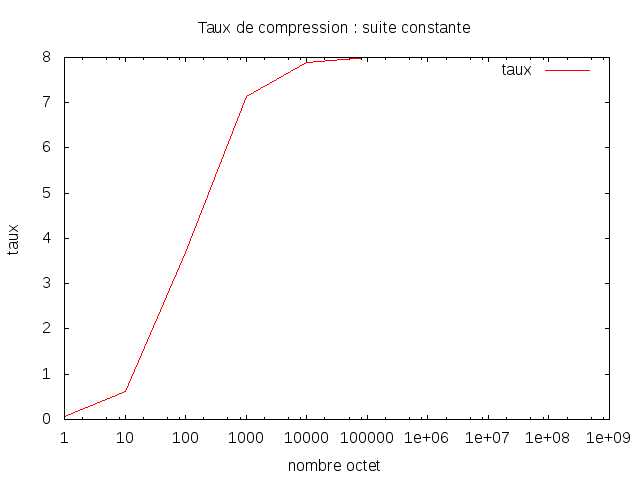
\includegraphics[width=11cm]{HConstant.png}

\end{center}



\subsubsection{ Analyse de l'agorithme de Lemple Ziv}

Tout d'abord regardons nos fichiers composés que de 0, nous obtenons le graphique ci-dessus.
\begin{center}

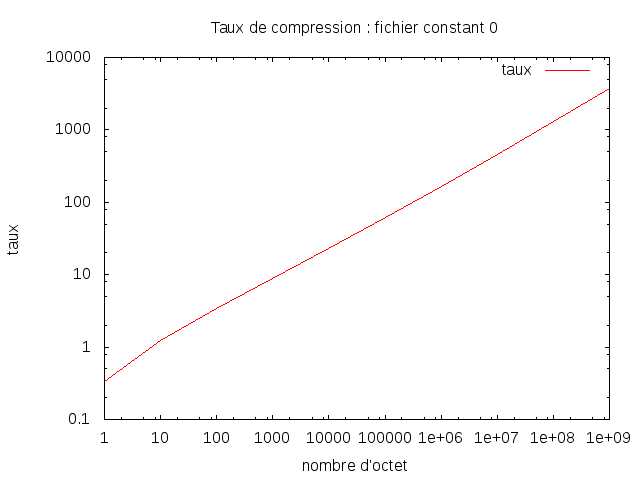
\includegraphics[width=11cm]{LZConstant.png}

\end{center}

On constate que la courbe est logarithmique, plus le nombre d'octet est important plus le taux de compression augmente, ainsi le fichier compressé devient réellement de plus en plus petit. 
On remarque néanmoins que lorsque l'on veut compresser un seul octet le taux de compression est en dessous de 1, c'est-à-dire que le fichier compressé est plus gros que le fichier source. Ceci s'explique notamment par le stockage du premier  octet supplémentaire pour connaître le mode de compression, ici Lempel-Ziv. Il s'explique aussi car le début de compression pour Lempel-Ziv remplace un bit par 2 et ainsi de suite. Nous devons donc attendre les 10 octets dans le fichier source pour que la compression ai vraiment lieu. 

\begin{center}

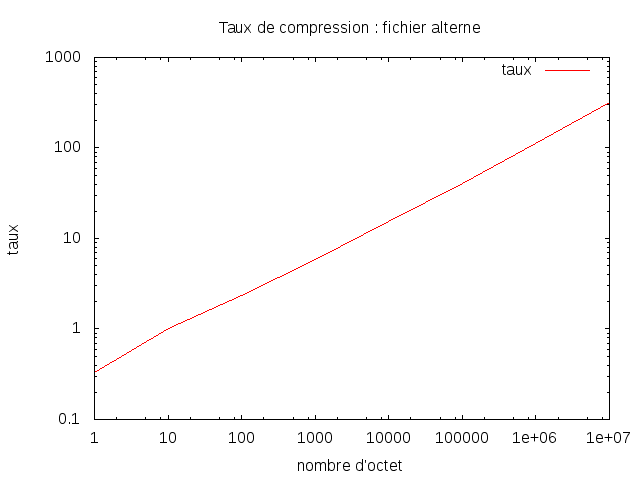
\includegraphics[width=11cm]{LZAlterner.png}

\end{center}

POur la suite alterner....
\begin{center}

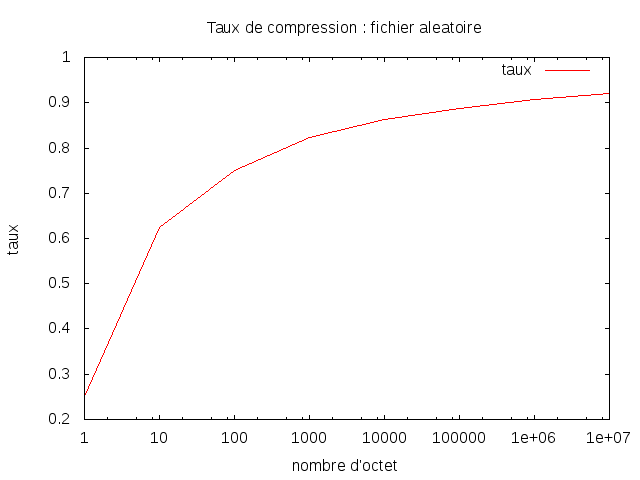
\includegraphics[width=11cm]{LZAleatoire.png}

\end{center}


\section*{Analyse du temps d’exécution}
\subsubsection*{Temps d’exécution pour la compression}
\subsubsection*{Temps d’exécution pour la décompression}


\section*{Différences entre les algorithmes}
Dans cette dernière section, nous allons vous présenter un tableau avec plusieurs mode de compression et plusieurs type de fichiers. 
Nous expliquerons par la suite les différents taux de compression obtenues. 


\begin{center}
{\renewcommand{\arraystretch}{2}
\begin{tabular}{|p{1.5cm}|p{1.5cm}|p{1.5cm}|p{1.5cm}|p{1.5cm}|p{1.5cm}|p{1.5cm}|p{1.5cm}|}
\hline
 & La bible (en anglais)  & Les Fleurs du Mal  & Au bonheurs des Dames & fichier PDF & musique  MP3 & image JPEG  \\
\hline
taille réélle (en octet)  & 883 158 & 180 199 & 952 753 &  & & \\\hline
zip & 3.44  & 2.51 & 2.57 & & & \\
\hline
Gzip & & & & & & \\
\hline
tar & & & & & & \\
\hline
Huffman & & & & & & \\
\hline
Lempel-Ziv & & & & & & \\
\hline

\end{tabular}
}
\end{center}




\end{document}
